\documentclass[border=10pt]{standalone}
\usepackage{tikz}
% Improve font rendering and switch to a clean sans-serif face
\usepackage[T1]{fontenc}
\usepackage{tgheros}
\renewcommand{\familydefault}{\sfdefault}
\usepackage{inconsolata}
\usetikzlibrary{shapes.geometric, arrows.meta, positioning, fit, backgrounds, shadows, patterns}

\begin{document}

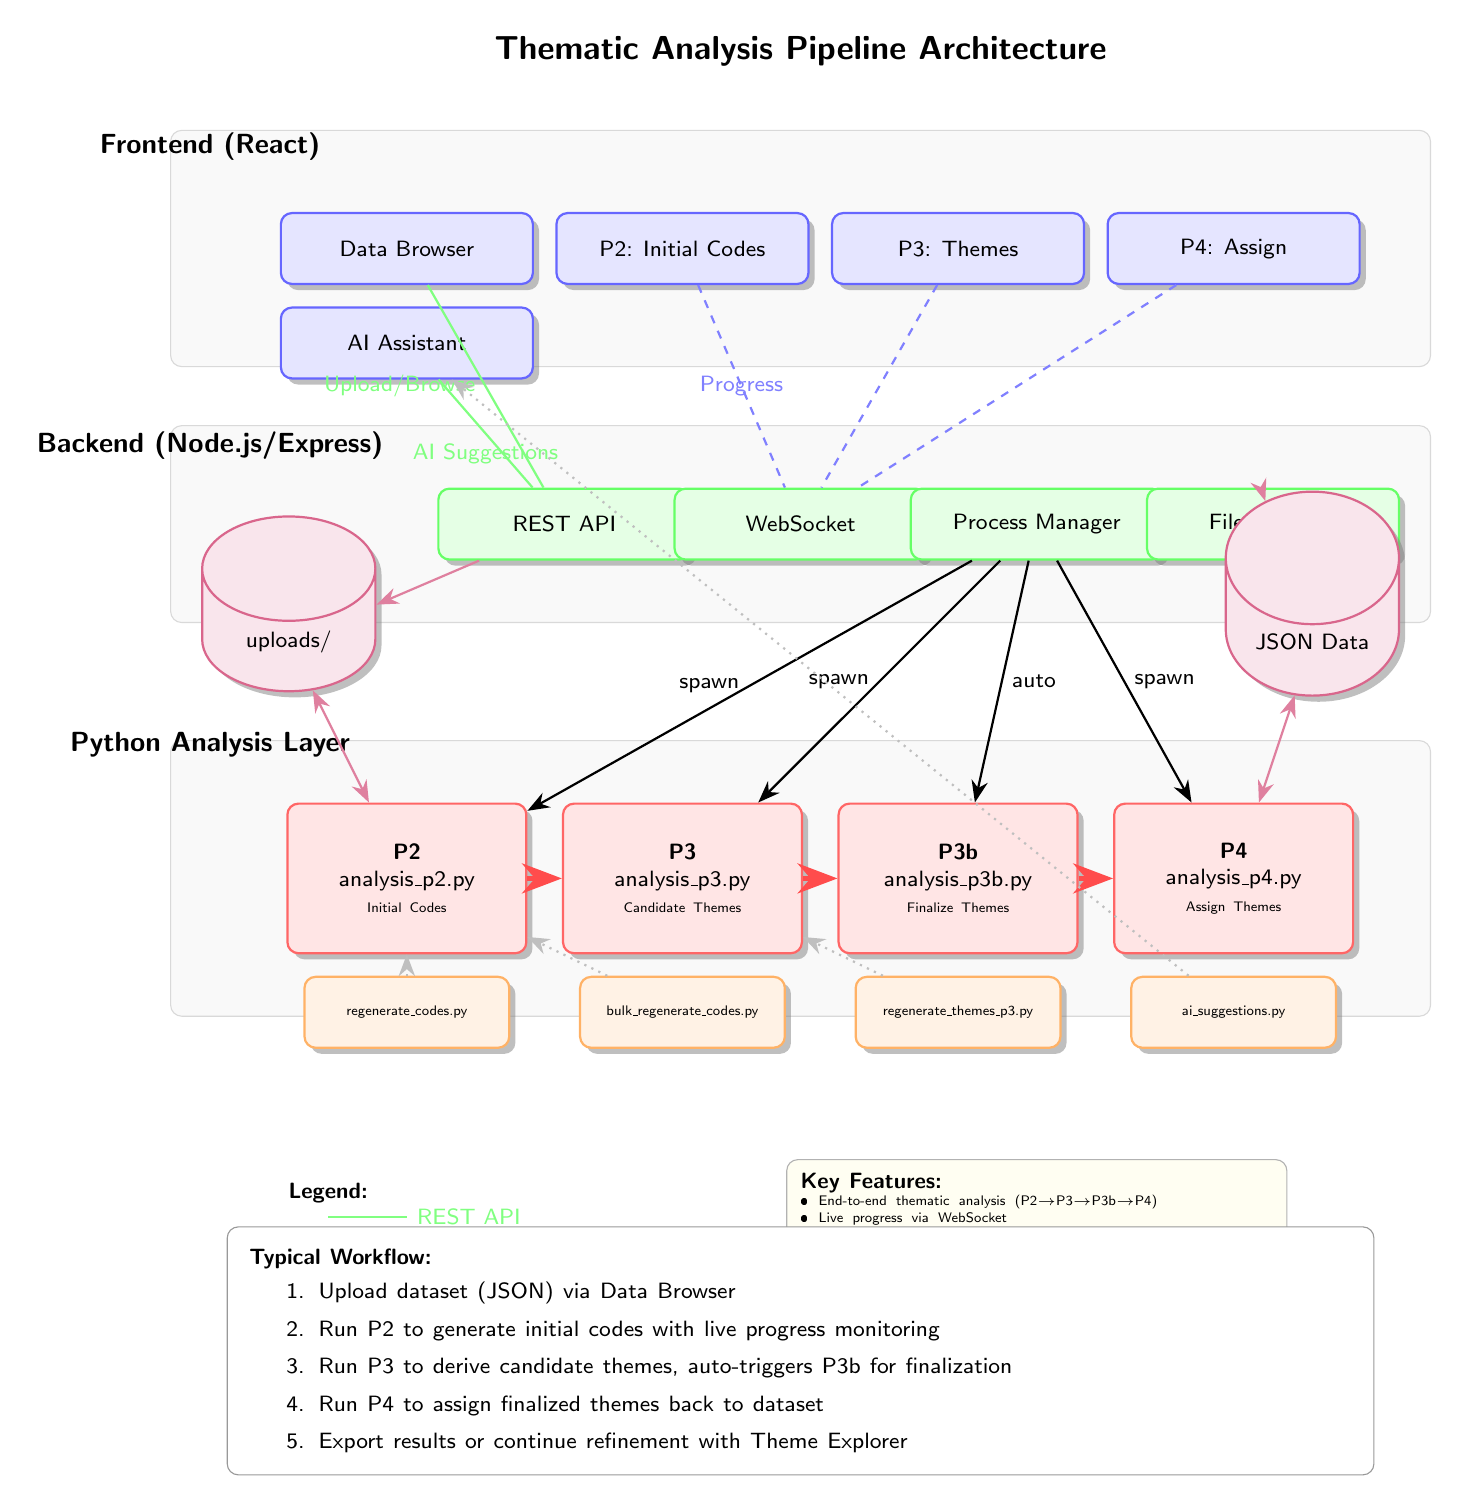
\begin{tikzpicture}[
    % Node styles
    frontend/.style={rectangle, draw=blue!60, fill=blue!10, line width=0.8pt,
        minimum width=3.2cm, minimum height=0.9cm, rounded corners, drop shadow,
        align=center, font=\sffamily\footnotesize},
    backend/.style={rectangle, draw=green!60, fill=green!10, line width=0.8pt,
        minimum width=3.2cm, minimum height=0.9cm, rounded corners, drop shadow,
        align=center, font=\sffamily\footnotesize},
    python/.style={rectangle, draw=orange!60, fill=orange!10, line width=0.8pt,
        minimum width=2.6cm, minimum height=0.9cm, rounded corners, drop shadow,
        align=center, font=\sffamily\footnotesize},
    data/.style={cylinder, draw=purple!60, fill=purple!10, line width=0.8pt,
        minimum width=2.2cm, minimum height=1.1cm, shape border rotate=90, drop shadow,
        align=center, font=\sffamily\footnotesize},
    phase/.style={rectangle, draw=red!60, fill=red!10, line width=0.8pt,
        minimum width=2.8cm, minimum height=1.9cm, text width=2.8cm,
        rounded corners, drop shadow, align=center, font=\sffamily\footnotesize},
    arrow/.style={-{Stealth[scale=1.2]}, thick},
    doublearrow/.style={{Stealth[scale=1.2]}-{Stealth[scale=1.2]}, thick},
    websocket/.style={dashed, thick, blue!50},
    rest/.style={solid, thick, green!50},
    label/.style={font=\footnotesize\sffamily},
    title/.style={font=\large\bfseries\sffamily},
    tier/.style={draw=gray!30, fill=gray!5, rounded corners, inner sep=10pt}
]

% Title
\node[title] at (0, 11) {Thematic Analysis Pipeline Architecture};

% Tier backgrounds
\begin{scope}[on background layer]
    \node[tier, minimum width=16cm, minimum height=3cm] (fronttier) at (0, 8.5) {};
    \node[tier, minimum width=16cm, minimum height=2.5cm] (backtier) at (0, 5) {};
    \node[tier, minimum width=16cm, minimum height=3.5cm] (pythontier) at (0, 0.5) {};
\end{scope}

% Tier labels
\node[label, font=\bfseries] at (-7.5, 9.8) {Frontend (React)};
\node[label, font=\bfseries] at (-7.5, 6) {Backend (Node.js/Express)};
\node[label, font=\bfseries] at (-7.5, 2.2) {Python Analysis Layer};

% Frontend components
\node[frontend] (databrowser) at (-5, 8.5) {Data Browser};
\node[frontend] (p2ui) at (-1.5, 8.5) {P2: Initial Codes};
\node[frontend] (p3ui) at (2, 8.5) {P3: Themes};
\node[frontend] (p4ui) at (5.5, 8.5) {P4: Assign};
\node[frontend] (ai) at (-5, 7.3) {AI Assistant};

% Backend components
\node[backend] (rest) at (-3, 5) {REST API};
\node[backend] (websocket) at (0, 5) {WebSocket};
\node[backend] (process) at (3, 5) {Process Manager};
\node[backend] (filemanager) at (6, 5) {File Manager};

% Data storage
\node[data] (uploads) at (-6.5, 3.5) {uploads/};
\node[data] (datafiles) at (6.5, 3.5) {JSON Data};

% Python scripts - Main pipeline
\node[phase] (p2) at (-5, 0.5) {\textbf{P2}\\\footnotesize analysis\_p2.py\\\tiny Initial Codes};
\node[phase] (p3) at (-1.5, 0.5) {\textbf{P3}\\\footnotesize analysis\_p3.py\\\tiny Candidate Themes};
\node[phase] (p3b) at (2, 0.5) {\textbf{P3b}\\\footnotesize analysis\_p3b.py\\\tiny Finalize Themes};
\node[phase] (p4) at (5.5, 0.5) {\textbf{P4}\\\footnotesize analysis\_p4.py\\\tiny Assign Themes};

% Python helper scripts
\node[python, font=\tiny] (regen1) at (-5, -1.2) {regenerate\_codes.py};
\node[python, font=\tiny] (regen2) at (-1.5, -1.2) {bulk\_regenerate\_codes.py};
\node[python, font=\tiny] (regen3) at (2, -1.2) {regenerate\_themes\_p3.py};
\node[python, font=\tiny] (aipy) at (5.5, -1.2) {ai\_suggestions.py};

% Arrows - Frontend to Backend
\draw[rest] (databrowser) -- (rest) node[midway, left, label] {Upload/Browse};
\draw[websocket] (p2ui) -- (websocket) node[midway, label] {Progress};
\draw[websocket] (p3ui) -- (websocket);
\draw[websocket] (p4ui) -- (websocket);
\draw[rest] (ai) -- (rest) node[midway, below, label] {AI Suggestions};

% Arrows - Backend to Python
\draw[arrow] (process) -- (p2) node[midway, left, label] {spawn};
\draw[arrow] (process) -- (p3) node[midway, left, label] {spawn};
\draw[arrow] (process) -- (p3b) node[midway, right, label] {auto};
\draw[arrow] (process) -- (p4) node[midway, right, label] {spawn};

% Pipeline flow
\draw[arrow, red!70, line width=2pt] (p2.east) -- (p3.west);
\draw[arrow, red!70, line width=2pt] (p3.east) -- (p3b.west);
\draw[arrow, red!70, line width=2pt] (p3b.east) -- (p4.west);

% Data connections
\draw[doublearrow, purple!50] (uploads) -- (p2);
\draw[doublearrow, purple!50] (datafiles) -- (p4);
\draw[arrow, purple!50] (filemanager) -- (datafiles);
\draw[arrow, purple!50] (rest) -- (uploads);

% Helper script connections
\draw[arrow, gray!50, dotted] (regen1) -- (p2);
\draw[arrow, gray!50, dotted] (regen2) -- (p2);
\draw[arrow, gray!50, dotted] (regen3) -- (p3);
\draw[arrow, gray!50, dotted] (aipy) -- (ai);

% Legend
\begin{scope}[shift={(0,-3.5)}]
    \node[label, font=\footnotesize\bfseries] at (-6, 0) {Legend:};
    \draw[rest] (-6, -0.3) -- (-5, -0.3) node[right, label] {REST API};
    \draw[websocket] (-6, -0.6) -- (-5, -0.6) node[right, label] {WebSocket};
    \draw[arrow, red!70, line width=2pt] (-6, -0.9) -- (-5, -0.9) node[right, label] {Pipeline Flow};
    \draw[arrow, gray!50, dotted] (-6, -1.2) -- (-5, -1.2) node[right, label] {Helper Scripts};
    
    % Key features box
    \node[draw=black!30, fill=yellow!5, rounded corners, text width=6cm, inner sep=5pt] at (3, -0.6) {
        \footnotesize\textbf{Key Features:}\\
        \tiny \textbullet{} End-to-end thematic analysis (P2\(\rightarrow\)P3\(\rightarrow\)P3b\(\rightarrow\)P4)\\
        \textbullet{} Live progress via WebSocket\\
        \textbullet{} Model selection (GPT-5/Gemini)\\
        \textbullet{} Per-case editing and regeneration\\
        \textbullet{} Theme organization and export\\
        \textbullet{} AI-powered suggestions
    };
\end{scope}

% Workflow annotation
\node[draw=black!40, fill=white, rounded corners, text width=14cm, inner sep=8pt] at (0, -5.5) {
    \footnotesize\textbf{Typical Workflow:}
    \begin{enumerate}
        \item Upload dataset (JSON) via Data Browser
        \item Run P2 to generate initial codes with live progress monitoring
        \item Run P3 to derive candidate themes, auto-triggers P3b for finalization
        \item Run P4 to assign finalized themes back to dataset
        \item Export results or continue refinement with Theme Explorer
    \end{enumerate}
};

\end{tikzpicture}

\end{document}